Le package render contient le code de l'interface graphique c'est à dire celui permettant l'affichage du rendu et des fenêtres.

\begin{description}
    \item [MainApp] contient le main de l'application et lance toutes les fenêtres.
    \item [SetSizeWindow] est la classe responsable de la fenêtre du choix de taille du rendu.
    \item [ImageWriter] est la classe responsable de l'affichage de la fenêtre du rendu.
    \item [Toolbox] est la classe responsable de la fenêtre de changement lors de l'affichage du rendu.
    \item [CameraTimer] est la classe responsable du déplacement de la caméra lors de l'appuie de touches.
    \item [Window Timer et CounterFPS] sont les classes responsable de l'affichage des FPS sur la fenêtre de rendu.
\end{description}



\begin{figure}[h]
   \caption{Fênetre de sélection de la taille du rendu}
   \begin{center}
       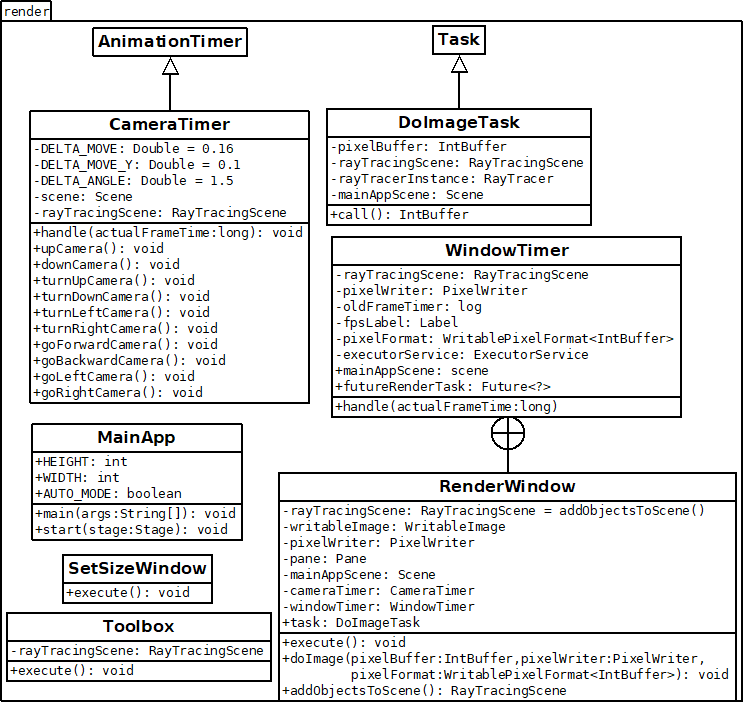
\includegraphics[scale=0.5]{img/render.javafx/diagClassRender.png}
   \end{center}
\end{figure}
